\documentclass[a4paper, 14pt]{extarticle}
\usepackage{float}
% Поля
%--------------------------------------
\usepackage{geometry}
\geometry{a4paper,tmargin=2cm,bmargin=2cm,lmargin=3cm,rmargin=1cm}
%--------------------------------------


%Russian-specific packages
%--------------------------------------
\usepackage[T2A]{fontenc}
\usepackage[utf8]{inputenc}
\usepackage[english, main=russian]{babel}
%--------------------------------------

\usepackage{textcomp}

% Красная строка
%--------------------------------------
\usepackage{indentfirst}
%--------------------------------------


%Graphics
%--------------------------------------
\usepackage{graphicx}
\graphicspath{ {./images/} }
\usepackage{wrapfig}
%--------------------------------------

% Полуторный интервал
%--------------------------------------
\linespread{1.3}
%--------------------------------------

%Выравнивание и переносы
%--------------------------------------
% Избавляемся от переполнений
\sloppy
% Запрещаем разрыв страницы после первой строки абзаца
\clubpenalty=10000
% Запрещаем разрыв страницы после последней строки абзаца
\widowpenalty=10000
%--------------------------------------

%Списки
\usepackage{enumitem}

%Подписи
\usepackage{caption}

%Гиперссылки
\usepackage{hyperref}

\hypersetup {
	unicode=true
}

%Рисунки
%--------------------------------------
\DeclareCaptionLabelSeparator*{emdash}{~--- }
\captionsetup[figure]{labelsep=emdash,font=onehalfspacing,position=bottom}
%--------------------------------------

\usepackage{tempora}

%Листинги
%--------------------------------------
\usepackage{listings}
\lstset{
  basicstyle=\ttfamily\footnotesize,
  %basicstyle=\footnotesize\AnkaCoder,        % the size of the fonts that are used for the code
  breakatwhitespace=false,        % sets if automatic breaks shoulbd only happen at whitespace
  breaklines=true,                 % sets automatic line breaking
  captionpos=t,                    % sets the caption-position to bottom
  inputencoding=utf8,
  frame=single,                    % adds a frame around the code
  keepspaces=true,                 % keeps spaces in text, useful for keeping indentation of code (possibly needs columns=flexible)
  keywordstyle=\bf,       % keyword style
  numbers=left,                    % where to put the line-numbers; possible values are (none, left, right)
  numbersep=5pt,                   % how far the line-numbers are from the code
  xleftmargin=25pt,
  xrightmargin=25pt,
  showspaces=false,                % show spaces everywhere adding particular underscores; it overrides 'showstringspaces'
  showstringspaces=false,          % underline spaces within strings only
  showtabs=false,                  % show tabs within strings adding particular underscores
  stepnumber=1,                    % the step between two line-numbers. If it's 1, each line will be numbered
  tabsize=2,                       % sets default tabsize to 8 spaces
  title=\lstname                   % show the filename of files included with \lstinputlisting; also try caption instead of title
}
%--------------------------------------

%%% Математические пакеты %%%
%--------------------------------------
\usepackage{amsthm,amsfonts,amsmath,amssymb,amscd}  % Математические дополнения от AMS
\usepackage{mathtools}                              % Добавляет окружение multlined
\usepackage[perpage]{footmisc}
%--------------------------------------

%--------------------------------------
%			НАЧАЛО ДОКУМЕНТА
%--------------------------------------

\begin{document}

%--------------------------------------
%			ТИТУЛЬНЫЙ ЛИСТ
%--------------------------------------
\begin{titlepage}
\thispagestyle{empty}
\newpage


%Шапка титульного листа
%--------------------------------------
\vspace*{-60pt}
\hspace{-65pt}
\begin{minipage}{0.3\textwidth}
\hspace*{-20pt}\centering

\includegraphics[width=\textwidth]{emblem}
\end{minipage}
\begin{minipage}{0.67\textwidth}\small \textbf{
\vspace*{-0.7ex}
\hspace*{-6pt}\centerline{Министерство науки и высшего образования Российской Федерации}
\vspace*{-0.7ex}
\centerline{Федеральное государственное бюджетное образовательное учреждение }
\vspace*{-0.7ex}
\centerline{высшего образования}
\vspace*{-0.7ex}
\centerline{<<Московский государственный технический университет}
\vspace*{-0.7ex}
\centerline{имени Н.Э. Баумана}
\vspace*{-0.7ex}
\centerline{(национальный исследовательский университет)>>}
\vspace*{-0.7ex}
\centerline{(МГТУ им. Н.Э. Баумана)}}
\end{minipage}
%--------------------------------------

%Полосы
%--------------------------------------
\vspace{-25pt}
\hspace{-35pt}\rule{\textwidth}{2.3pt}

\vspace*{-20.3pt}
\hspace{-35pt}\rule{\textwidth}{0.4pt}
%--------------------------------------

\vspace{1.5ex}
\hspace{-35pt} \noindent \small ФАКУЛЬТЕТ\hspace{80pt} <<Информатика и системы управления>>

\vspace*{-16pt}
\hspace{47pt}\rule{0.83\textwidth}{0.4pt}

\vspace{0.5ex}
\hspace{-35pt} \noindent \small КАФЕДРА\hspace{50pt} <<Теоретическая информатика и компьютерные технологии>>

\vspace*{-16pt}
\hspace{30pt}\rule{0.866\textwidth}{0.4pt}

\vspace{11em}

\begin{center}
\Large {\bf Лабораторная работа № 4.2} \\
\large {\bf по курсу <<Численные методы линейной алгебры>>} \\
\large <<Вычисление собственных значений и собственных
векторов симметричной матрицы методом А.Н. Крылова>>
\end{center}\normalsize

\vspace{8em}


\begin{flushright}
  {Студент группы ИУ9-71Б Баев Д.А \hspace*{15pt}\\
  \vspace{2ex}
  Преподаватель Посевин Д. П.\hspace*{15pt}}
\end{flushright}

\bigskip

\vfill


\begin{center}
\textsl{Москва 2023}
\end{center}
\end{titlepage}
%--------------------------------------
%		КОНЕЦ ТИТУЛЬНОГО ЛИСТА
%--------------------------------------

\renewcommand{\ttdefault}{pcr}

\setlength{\tabcolsep}{3pt}
\newpage
\setcounter{page}{2}

\section{Задание}\label{Sect::task}
1. Реализовать метод поиска собственных значений действительной
симметричной матрицы A размером 4х4.

2. Проверить корректность вычисления собственных значений по теореме
Виета.

3. Проверить выполнение условий теоремы Гершгорина о принадлежности
собственных значений соответствующим объединениям кругов
Гершгорина.

4. Вычислить собственные вектора и проверить выполнение условия
ортогональности собственных векторов.

5. Проверить решение на матрице приведенной в презентации.

6. Продемонстрировать работу приложения для произвольных
симметричных матриц размером n х n с учетом выполнения пунктов
приведенных выше.
\newpage
\section{Исходный код}

Исходный код программы представлен в листингах~\ref{lst:code1}--~\ref{lst:code4}.

\begin{figure}[H]
\begin{lstlisting}[language={},caption={Вычисление собственных значений и векторов со всеми проверками},label={lst:code1}]
def eig(A):
    assert len(A) == len(A[0])
    assert is_sym_matrix(A)
    n = len(A)
    intervals = gerchgoin_intervals(A)
    trace = sum(A[i][i] for i in range(n))
    coefs, B = danilevskiy(A)
    coefs = list(map(lambda x: x * -1, coefs))
    f = lambda x: np.polyval([1] + coefs, x)
    search_intervals = binary_search_intervals(intervals, f)
    eigs = binary_search_roots(search_intervals, f)
    check_gerchgoin(intervals, eigs)
    print(f"Viet theorem:\nSum = {sum(eigs)}\nTrace = {trace}")
    eig_vectors = []
    for eig in eigs:
        y_vector = [eig ** i for i in range(n - 1, -1, -1)]
        x_vector = np.array(mul_matrix_by_vector(B, y_vector))
        eig_vectors.append(x_vector / norm(x_vector))
    print("Ortnorm eig vectors:")
    print('Norms:')
    for vector in eig_vectors:
        print(norm(vector))
    print("Scalar prods:")
    for i in range(n - 1):
        for j in range(i + 1, n):
            print(scalar(eig_vectors[i], eig_vectors[j]))
    return np.array(eigs), eig_vectors
\end{lstlisting}
\end{figure}

\begin{figure}[H]
\begin{lstlisting}[language={},caption={Вычисление коофициентов характеристического уравнения и собственных векторов методом А.Н. Крылова},label={lst:code2}]
def krylov_eig_vectors(A, Y, coefs, eigs):
    n = len(A)
    Q = np.zeros(shape=(n, n))
    for i in range(n):
        for j in range(n):
           Q[j][i] = 1 if j == 0 else eigs[i] * Q[j - 1][i] + coefs[j - 1]
    vectors = []
    for i in range(n):
        vector = deepcopy(Y[0])
        for j in range(1, n):
            vector += Q[j][i] * Y[j]
        vectors.append(vector / norm(vector))
    return vectors


def krylov(A):
    n = len(A)
    y = np.random.uniform(-10, 10, n)
    Y = [y]
    for i in range(n - 1):
        y = mul_matrix_by_vector(A, y)
        Y.append(y)
    b = mul_matrix_by_vector(A, y)
    Y = np.array(list(reversed(Y)))
    P = Y.T
    coefs = np.linalg.solve(P, b)
    return coefs, Y
\end{lstlisting}
\end{figure}

\begin{figure}[H]
\begin{lstlisting}[language={},caption={Вычисление и объединение кругов Гершгорина},label={lst:code3}]
def gerchgoin_intervals(A):
    intervals = []
    for i in range(len(A)):
        center = A[i][i]
        radius = sum(abs(A[i][j]) for j in range(len(A)) if j != i)
        intervals.append([center - radius, center + radius])

    intervals.sort(key=lambda x:x[0])
    merged = [intervals[0]]
    for i in range(1, len(intervals)):
        current_interval = intervals[i]
        previous_interval = merged[-1]
        if current_interval[0] <= previous_interval[1]:
            merged[-1] = [previous_interval[0], max(previous_interval[1], current_interval[1])]
        else:
            merged.append(current_interval)

    return merged

def check_gerchgoin(intervals, eigs):
    for eig in eigs:
        interval_found = False
        for interval in intervals:
            if interval[0] <= eig <= interval[1]:
                interval_found = True
                break
        if not interval_found:
            print(f"Eig: {eig} not in gerchgoin circles")
            return
    print("All eigs in gerchgoin circles")
\end{lstlisting}
\end{figure}

\begin{figure}[H]
\begin{lstlisting}[language={},caption={Решение характеристического уравнения методом бинарного поиска},label={lst:code4}]
def binary_search_roots(intervals, f, delta=1e-3):
    lambdas = []
    for interval in intervals:
        left = interval[0]
        right = interval[1]
        f_left = f(left)
        assert f_left * f(right) < 0
        x = (left + right) / 2
        f_x = f(x)
        while abs(f_x) > delta:
            if f_left * f_x < 0:
                right = x
            else:
                left = x
                f_left = f(left)
            x = (left + right) / 2
            if x == left or x == right:
                break
            f_x = f(x)
        lambdas.append(x)
    return lambdas

def binary_search_intervals(intervals, f, delta=0.1):
    search_intervals = []
    for interval in intervals:
        left = interval[0]
        right = interval[1]
        delta_x = left + delta
        while delta_x <= right:
            f_left = f(left)
            f_delta = f(delta_x)
            if f_left * f_delta < 0:
                search_intervals.append([left, delta_x])
                left = delta_x
                delta_x = left + delta
            else:
                delta_x += delta
    return search_intervals
\end{lstlisting}
\end{figure}

\section{Результаты}

Результат поиска собственных значений и векторов и все необходимые проверки представлены на рисунках~\ref{fig:img1}-~\ref{fig:img3}.


\begin{figure}[H]
\centering
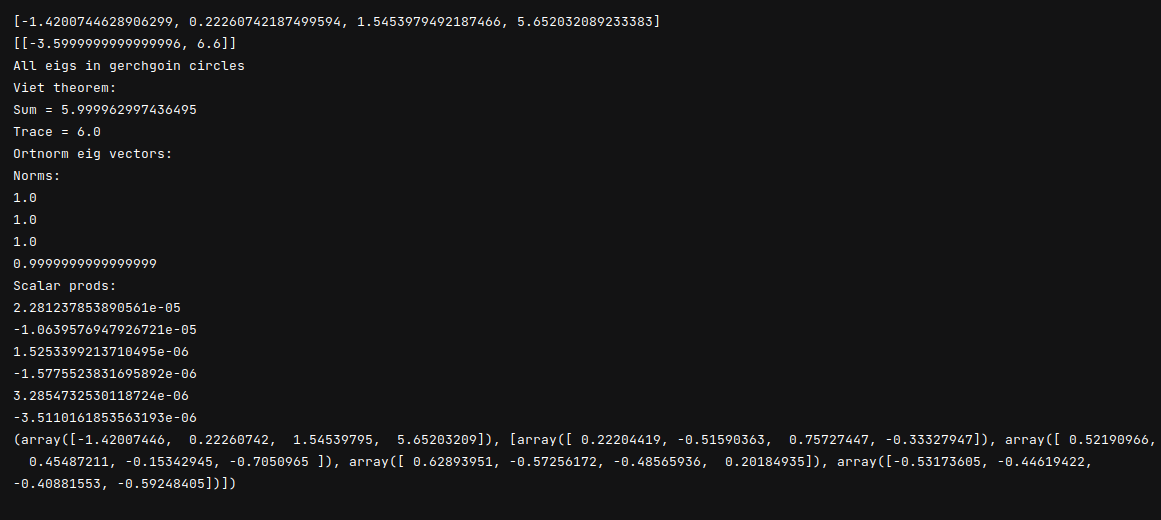
\includegraphics[width=0.8\textwidth]{images/res1.png}
\caption{Результат поиска собственных значений и векторов для матрицы 4x4 (из презентации)}
\label{fig:img1}
\end{figure}


\begin{figure}[H]
\centering
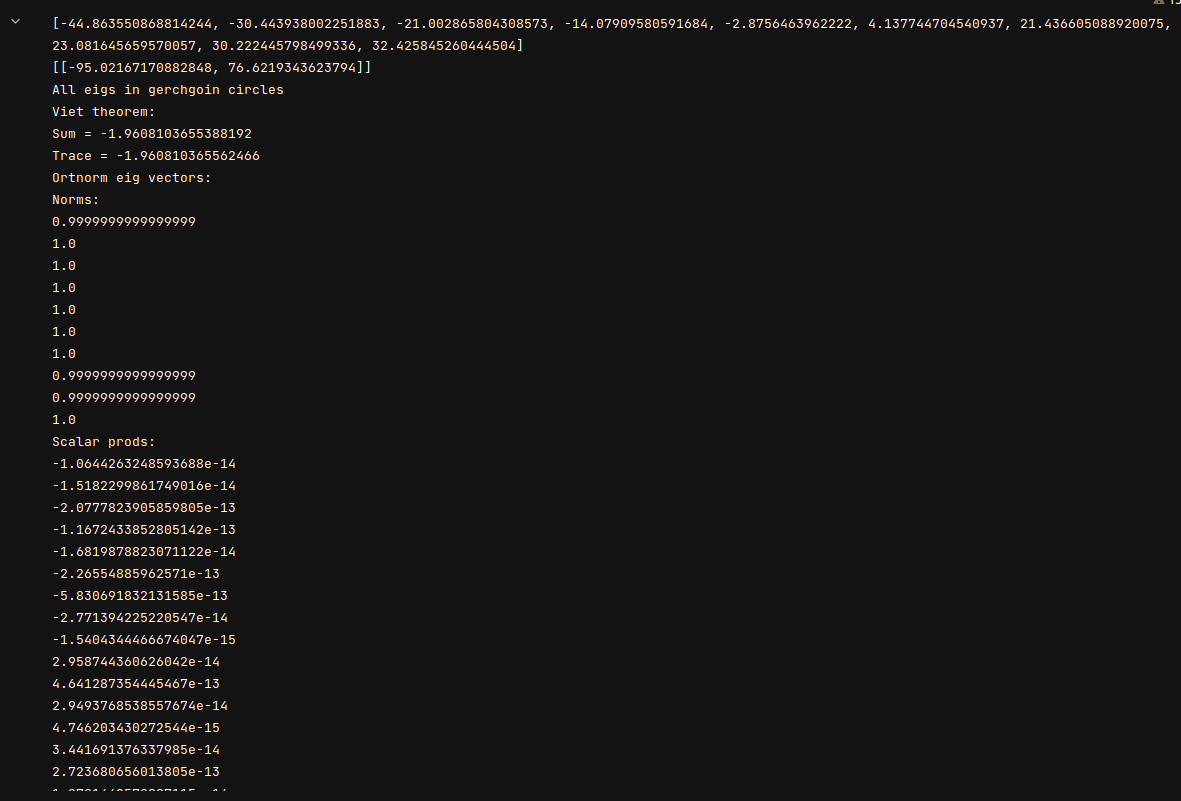
\includegraphics[width=0.8\textwidth]{images/res2.png}
\caption{Результат поиска собственных значений и векторов для произвольной матрицы 10x10}
\label{fig:img2}
\end{figure}


\begin{figure}[H]
\centering
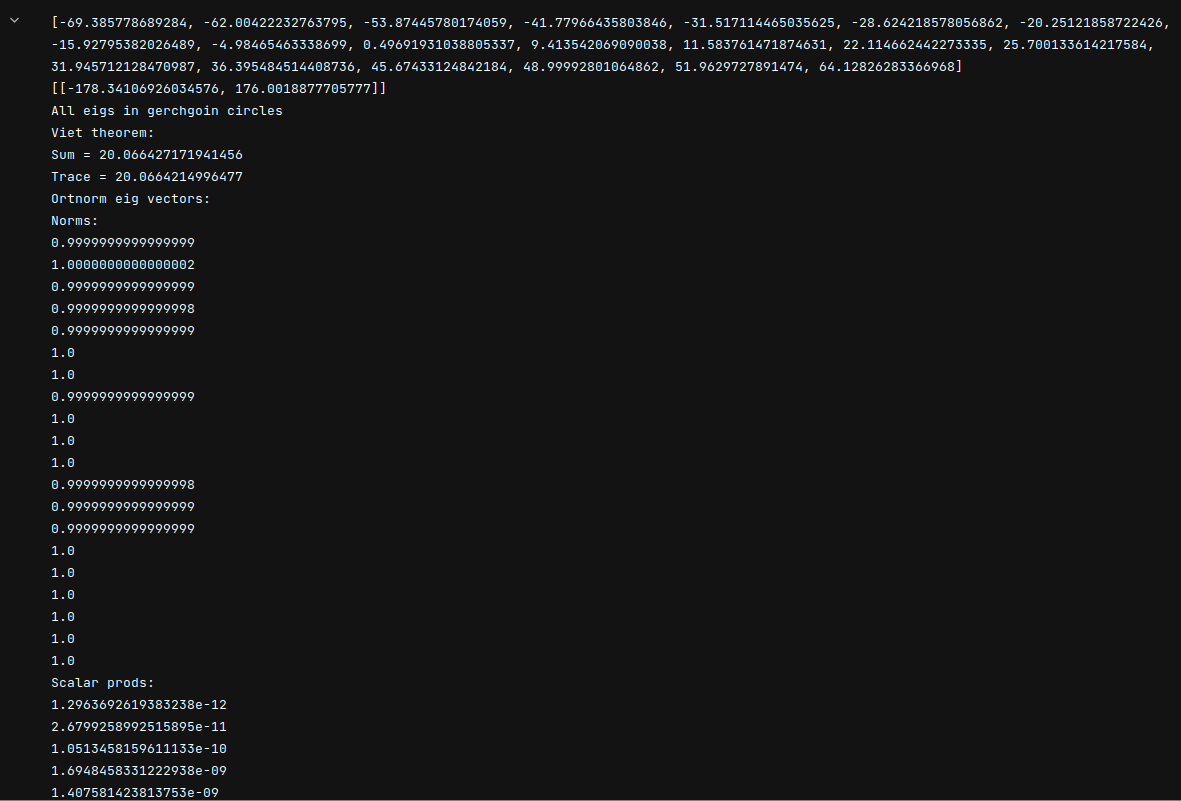
\includegraphics[width=0.8\textwidth]{images/res3.png}
\caption{Результат поиска собственных значений и векторов для произвольной матрицы 20x20}
\label{fig:img3}
\end{figure}


\section{Выводы}
В результате выполнения лабораторной работы был реализован метод для поиска собственных значений и нормированной системы собственных векторов произвольной квадратной действительной симметричной матрицы. Для поиска собственных значений метод использует метод бинарного поиска, локализуя область поиска с помощью теоремы Гершгорина. Коофициенты характеристического уравнения и собственные вектора вычисляются при помощи метода А.Н. Крылова.
\end{document}